\documentclass{nusthesis}

% --------------------------------------------------
% Basic information
% --------------------------------------------------
\title{Quad Polarization Wideband Sinuous Antenna Elements and Arrays}
\author{Ramanan Balakrishnan}
\qualification{B.Eng. (Hons.), NUS}

\degree{Master of Engineering}
\university{National University of Singapore}
\department{Department of Electrical and \\Computer Engineering}
\submityear{2015}

\date{\today}

\begin{document}

% --------------------------------------------------
% Build the cover page, title page, declaration,
% dedication and acknowledgement pages
% --------------------------------------------------
\frontmatter
\maketitle
\declarationpage{}

\newpage
\thispagestyle{empty}
\begin{flalign*}
&&\nabla \cdot \mathbf{E} &= \frac{\rho}{\epsilon_0 \nonumber}\\
&&\nabla \cdot \mathbf{B} &= 0 \nonumber \\
&&\nabla \times \mathbf{E} &= - \frac{\partial B}{\partial t} \nonumber \\
&&\nabla \times \mathbf{B} &= \mu_{0}\mathbf{J} + \mu_{0}\epsilon_{0}\frac{\partial E}{\partial t} \nonumber
\end{flalign*}
\hfill \emph{and there was light}

\newpage
\acknowledgment{
Let's thank some people here.
}

% --------------------------------------------------
% Table of contents, abstract,
% lists of tables, figures and symbols
% --------------------------------------------------
\tableofcontents
\newpage
\abstract{
A section to summarize the main contributions of this thesis.
}

\listoftables
\listoffigures
\listofsymbolsnabbrev

% --------------------------------------------------
% Main content of thesis organized into chapters
% --------------------------------------------------
\mainmatter

\chapter{The basics}
\label{chap:introduction}
And so it begins ...

\section{A simple section}
\label{sec:asimplesection}
A citation \cite{Hofstadter1979}. Here is another citation \cite{Balakrishnan2013}.

\subsection{A sub-section}
\label{ssec:asubsection}
Some more text here.

\chapter{Figures, sub-figures and more}
\label{chap:figures}

A simple figure called \cref{fig:example_fig} is shown below.

\begin{figure}[!htbp]
\centering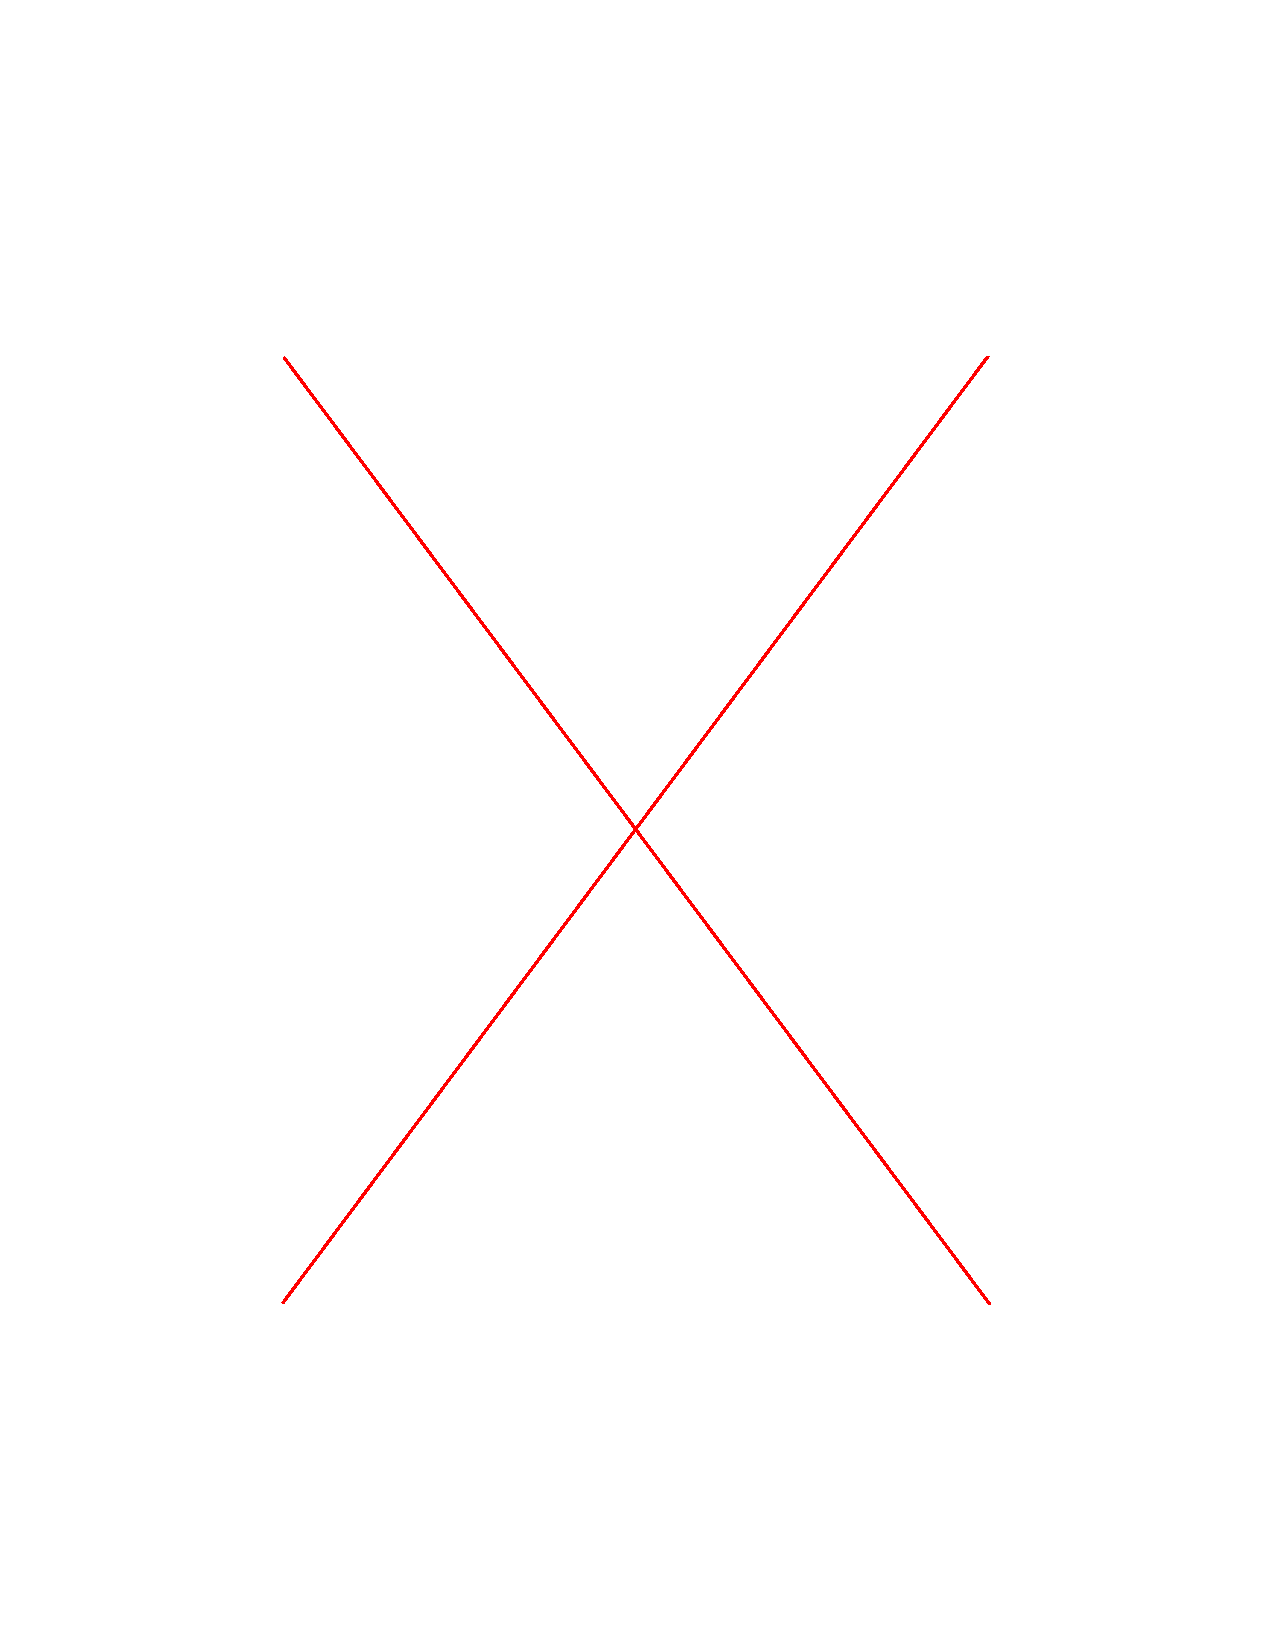
\includegraphics[width=0.5\textwidth]{fig}
\caption{Captions are also possible for figures.}
\label{fig:example_fig}
\end{figure}

\newpage

More complicated layouts of multiple figures using \texttt{subfloat} are also
possible as shown in \cref{fig:example_subfig}. Reference a subfigure directly
as \cref{subfig:subfig_1}.

\begin{figure}[!ht]
    \subfloat[ \label{subfig:subfig_1}]{%
     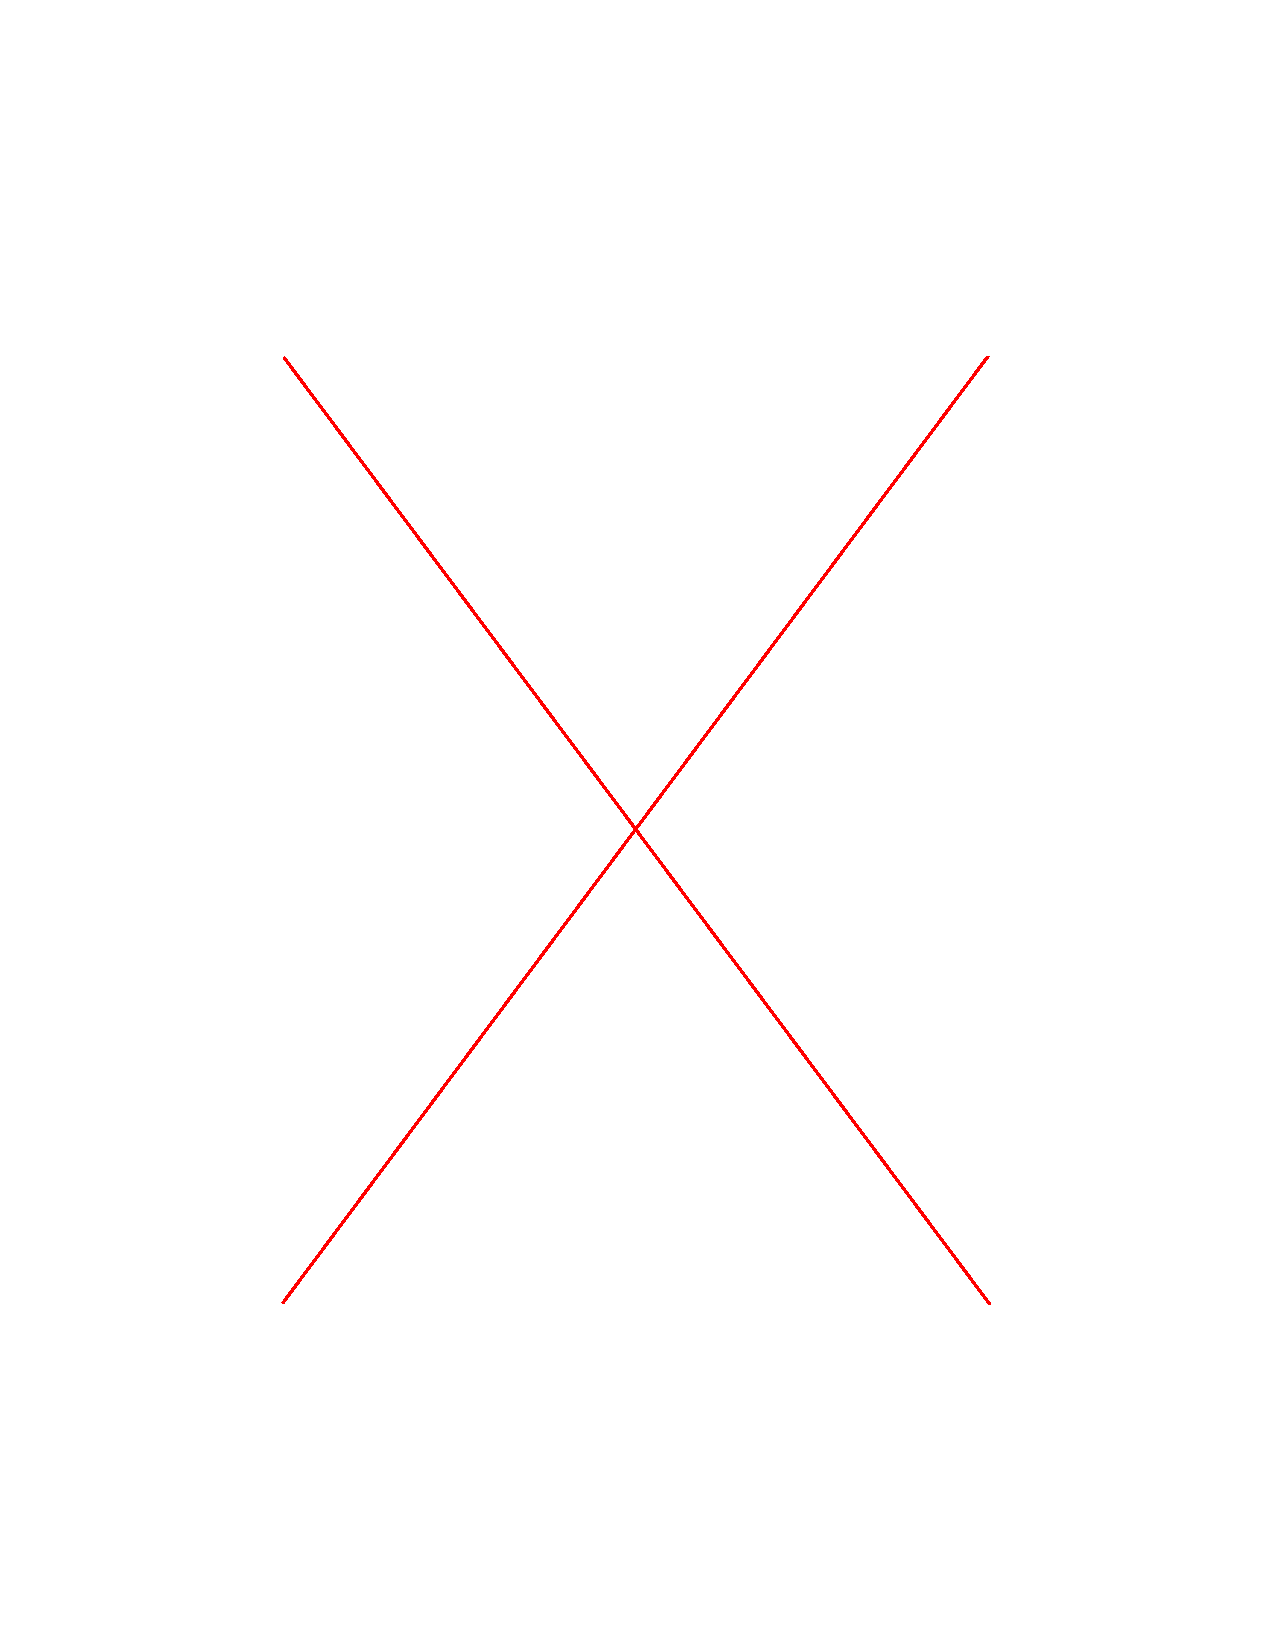
\includegraphics[width=0.3\textwidth]{small_fig}
   }
   \hfill
   \subfloat[ \label{subfig:subfig_2}]{%
     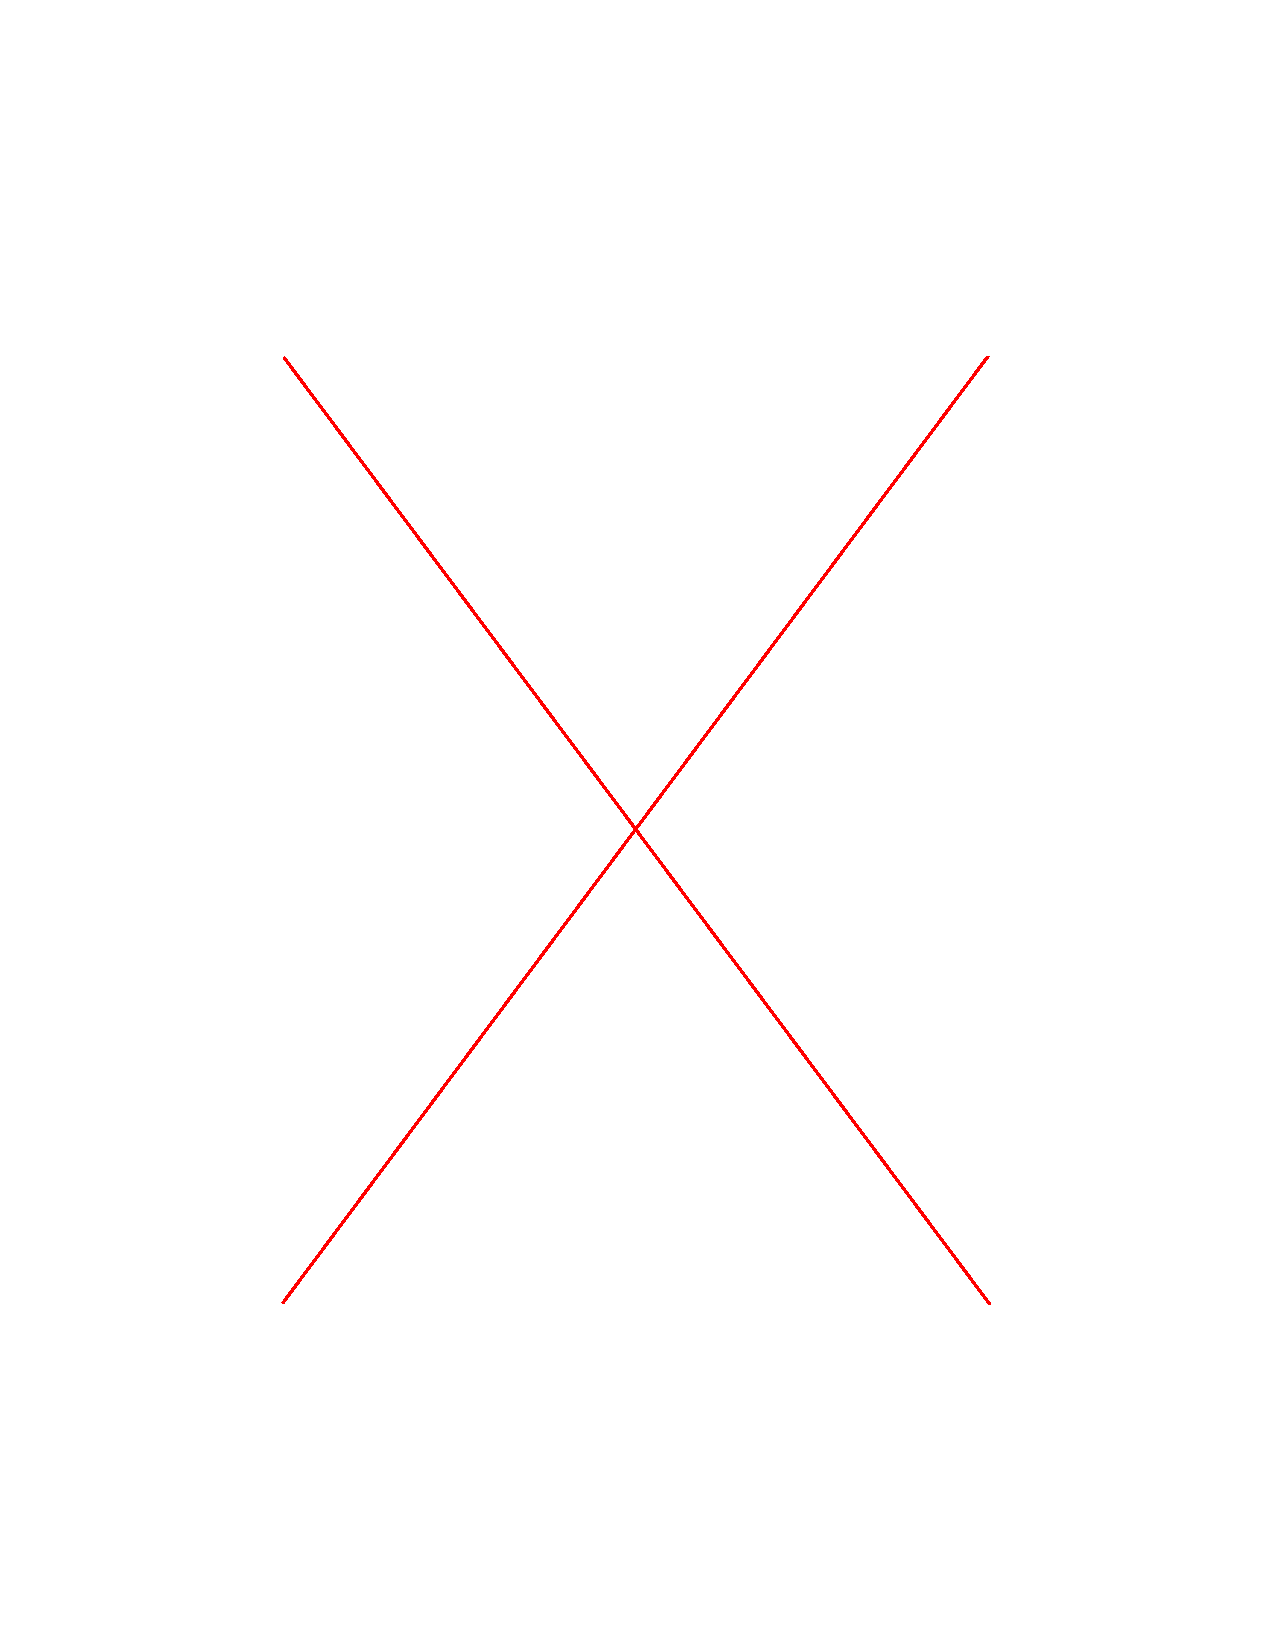
\includegraphics[width=0.3\textwidth]{small_fig}
   }
   \caption{A common caption is shown for both. Use (a) and (b) to refer to the
   subfigures.}
\label{fig:example_subfig}
\end{figure}

Finally, a full page of figures with a possible layout is shown in \cref{fig:full_page_fig}.

\begin{figure}[!htbp]
    \subfloat[]{ 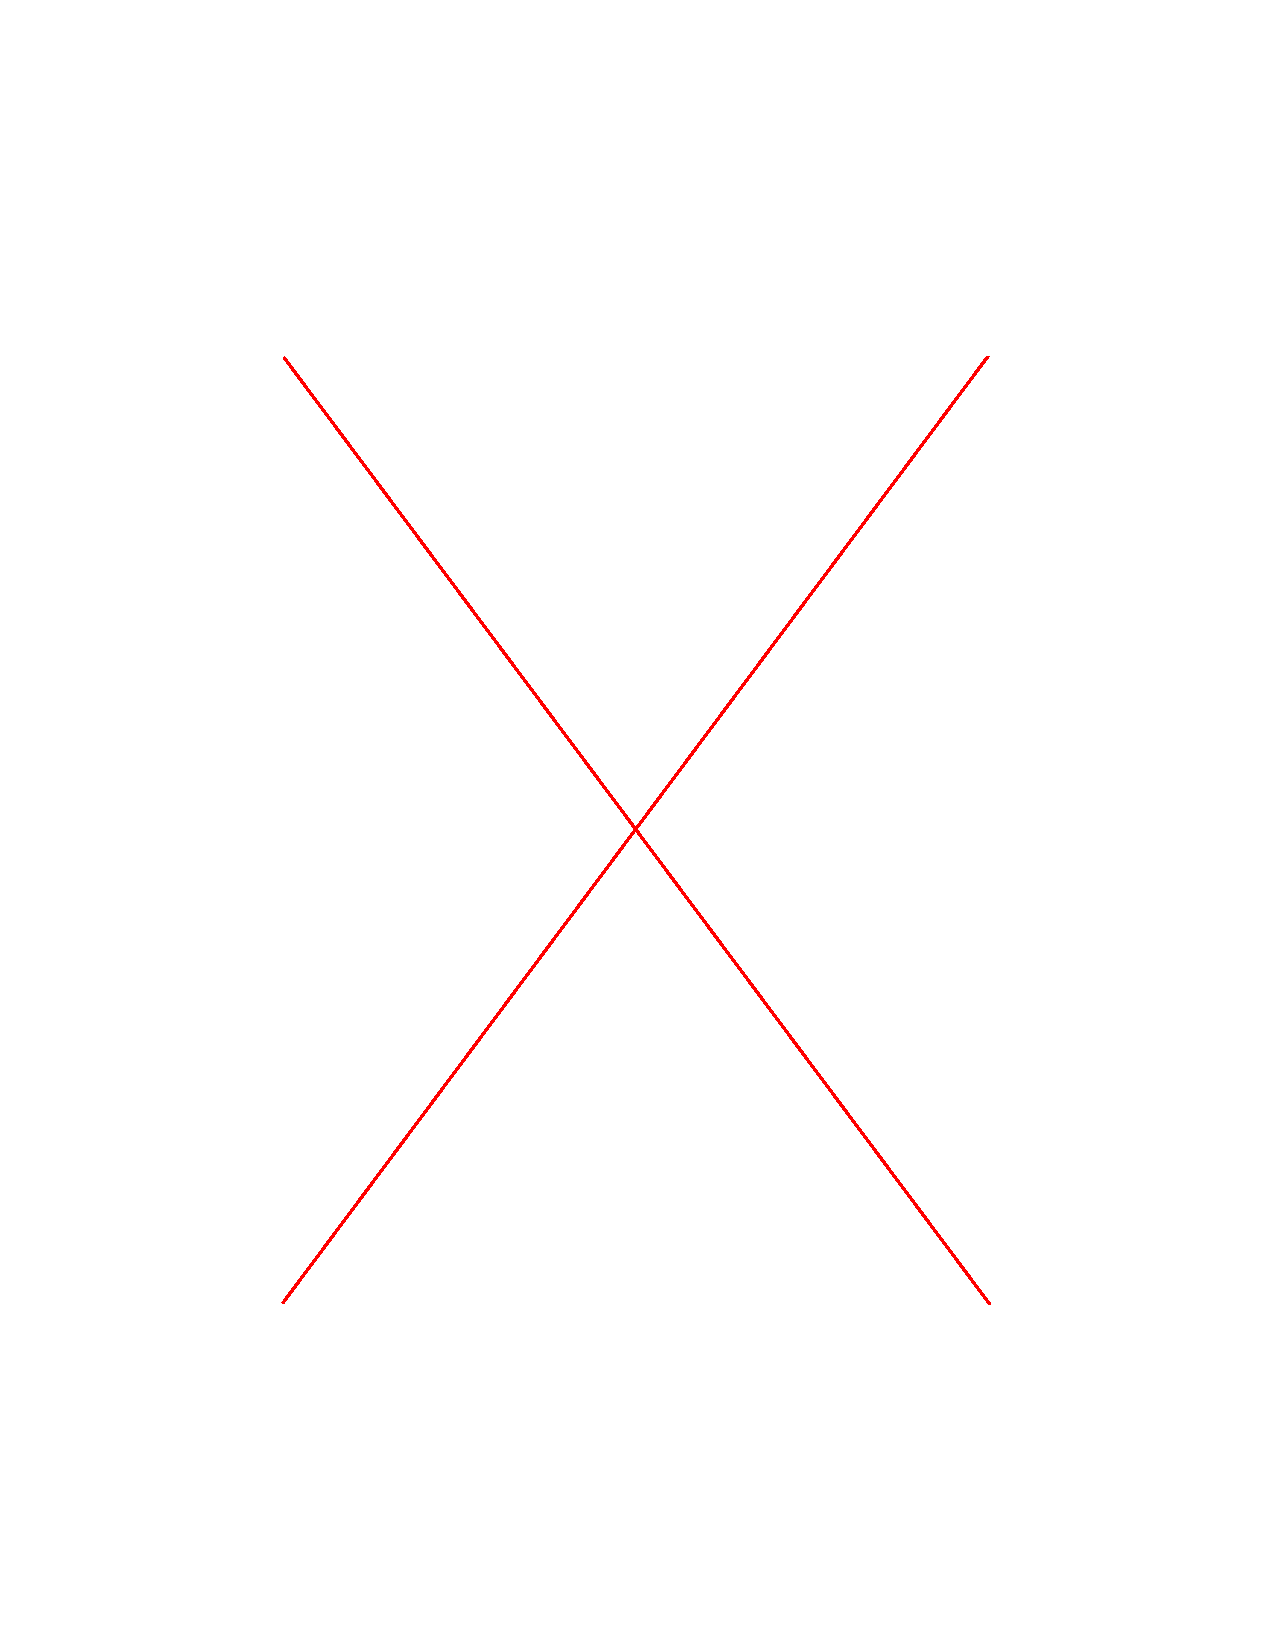
\includegraphics[width=0.4\textwidth]{small_fig} }
   \hfill
    \subfloat[]{ 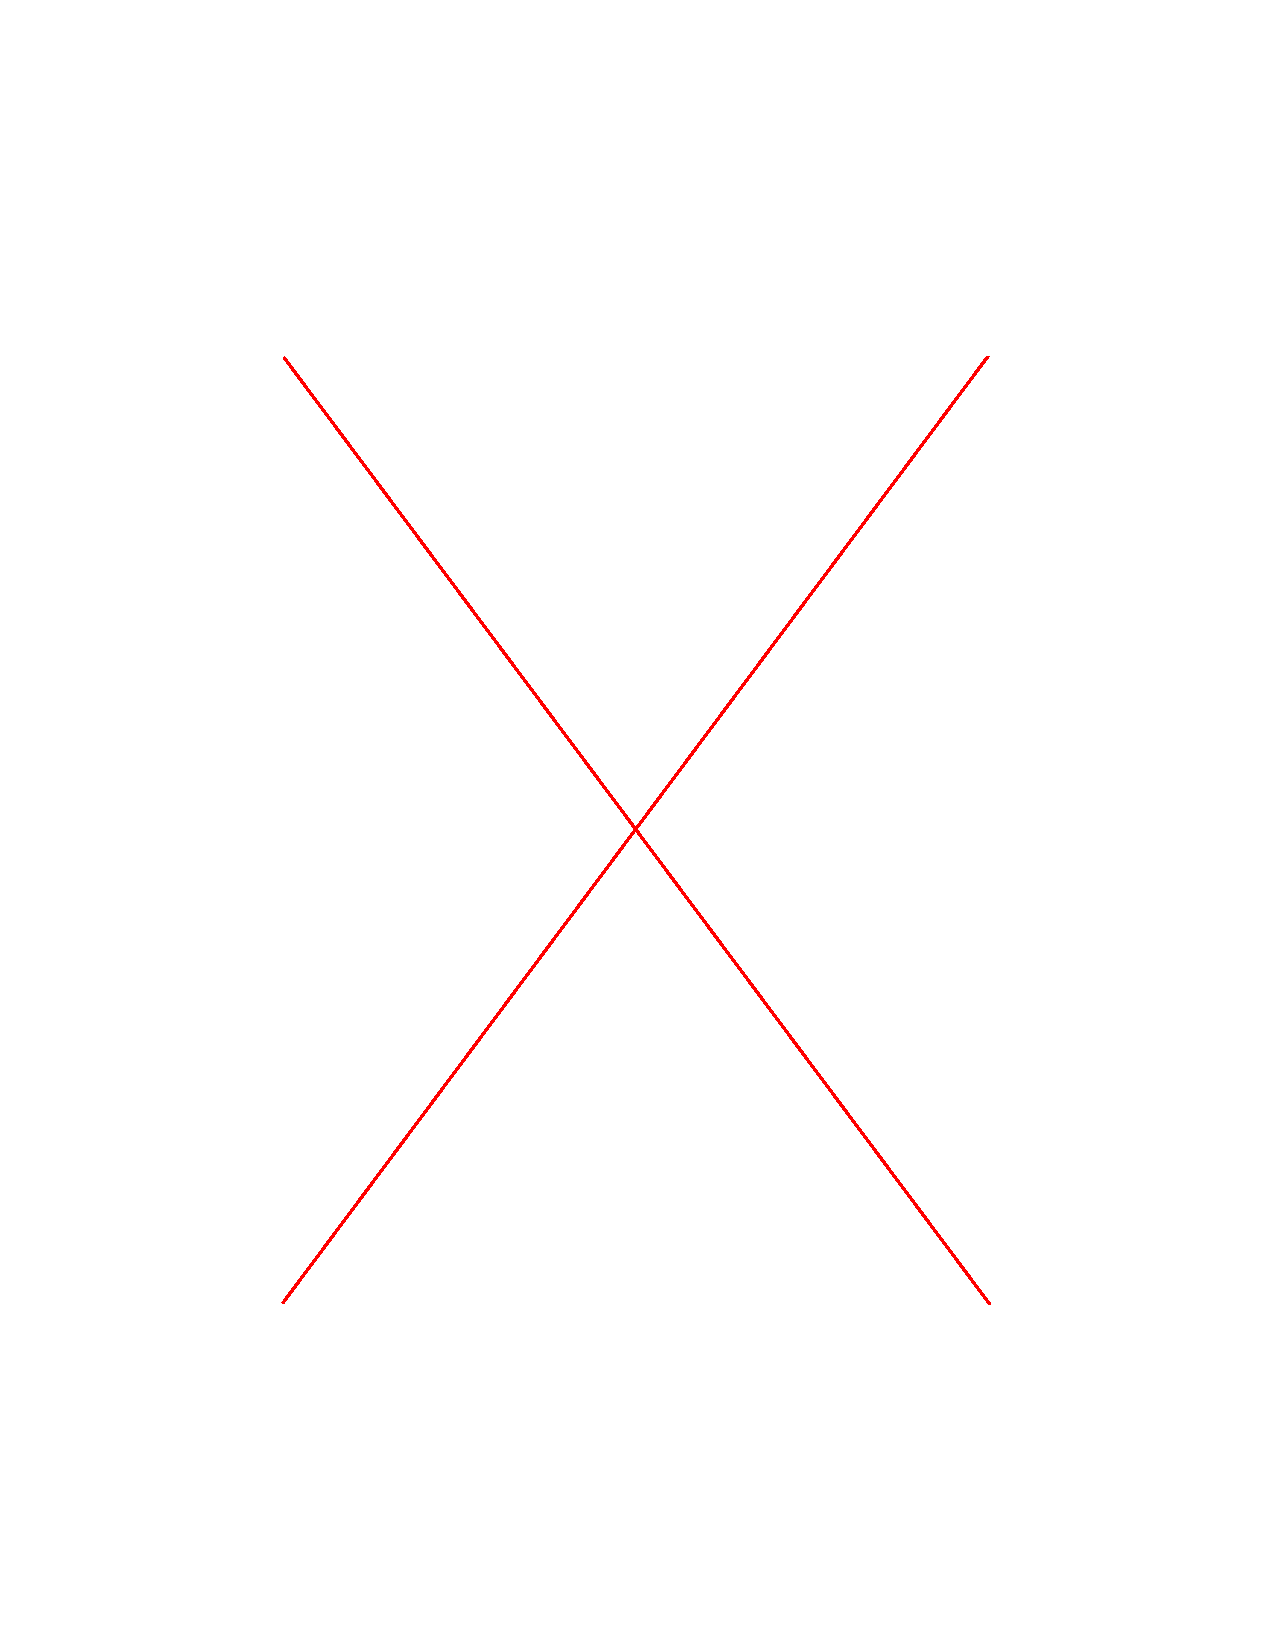
\includegraphics[width=0.4\textwidth]{small_fig} } \\
    \subfloat[]{ 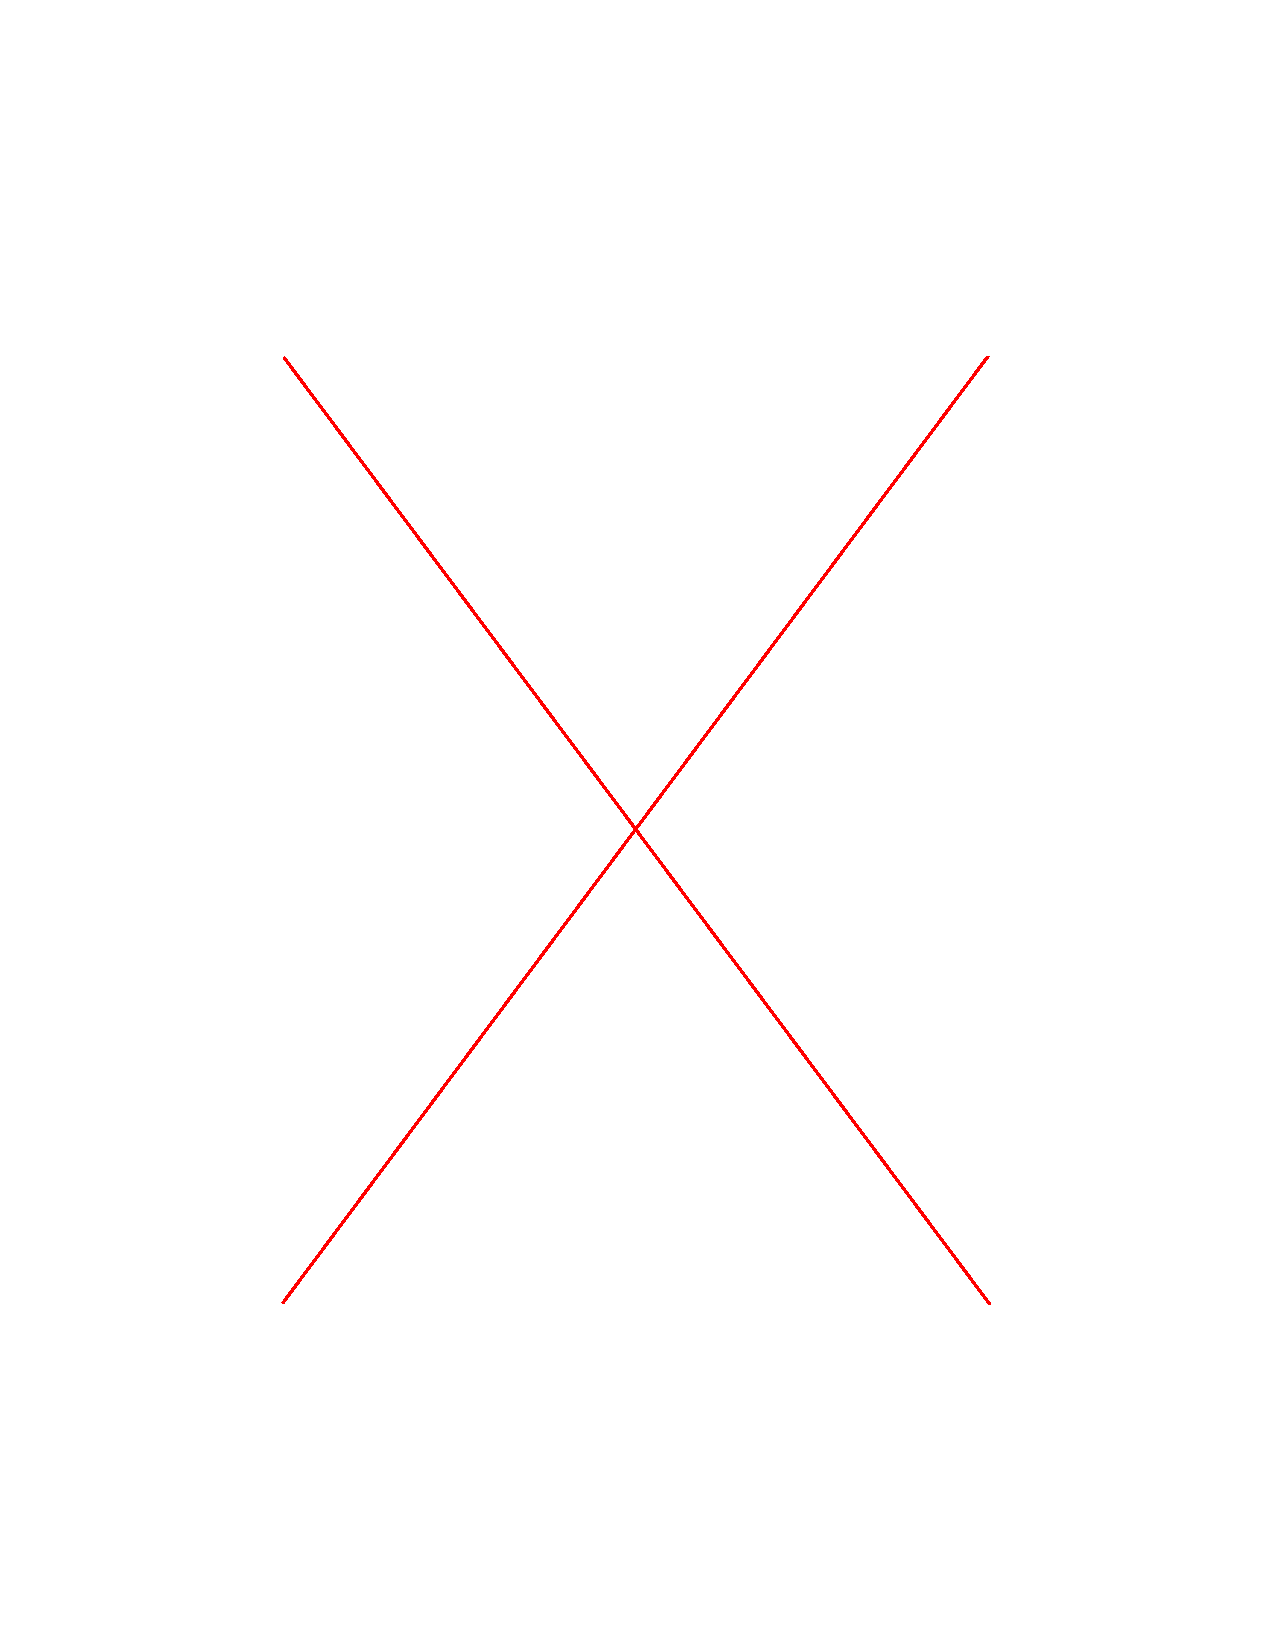
\includegraphics[width=0.4\textwidth]{small_fig} }
        \hfill
    \subfloat[]{ 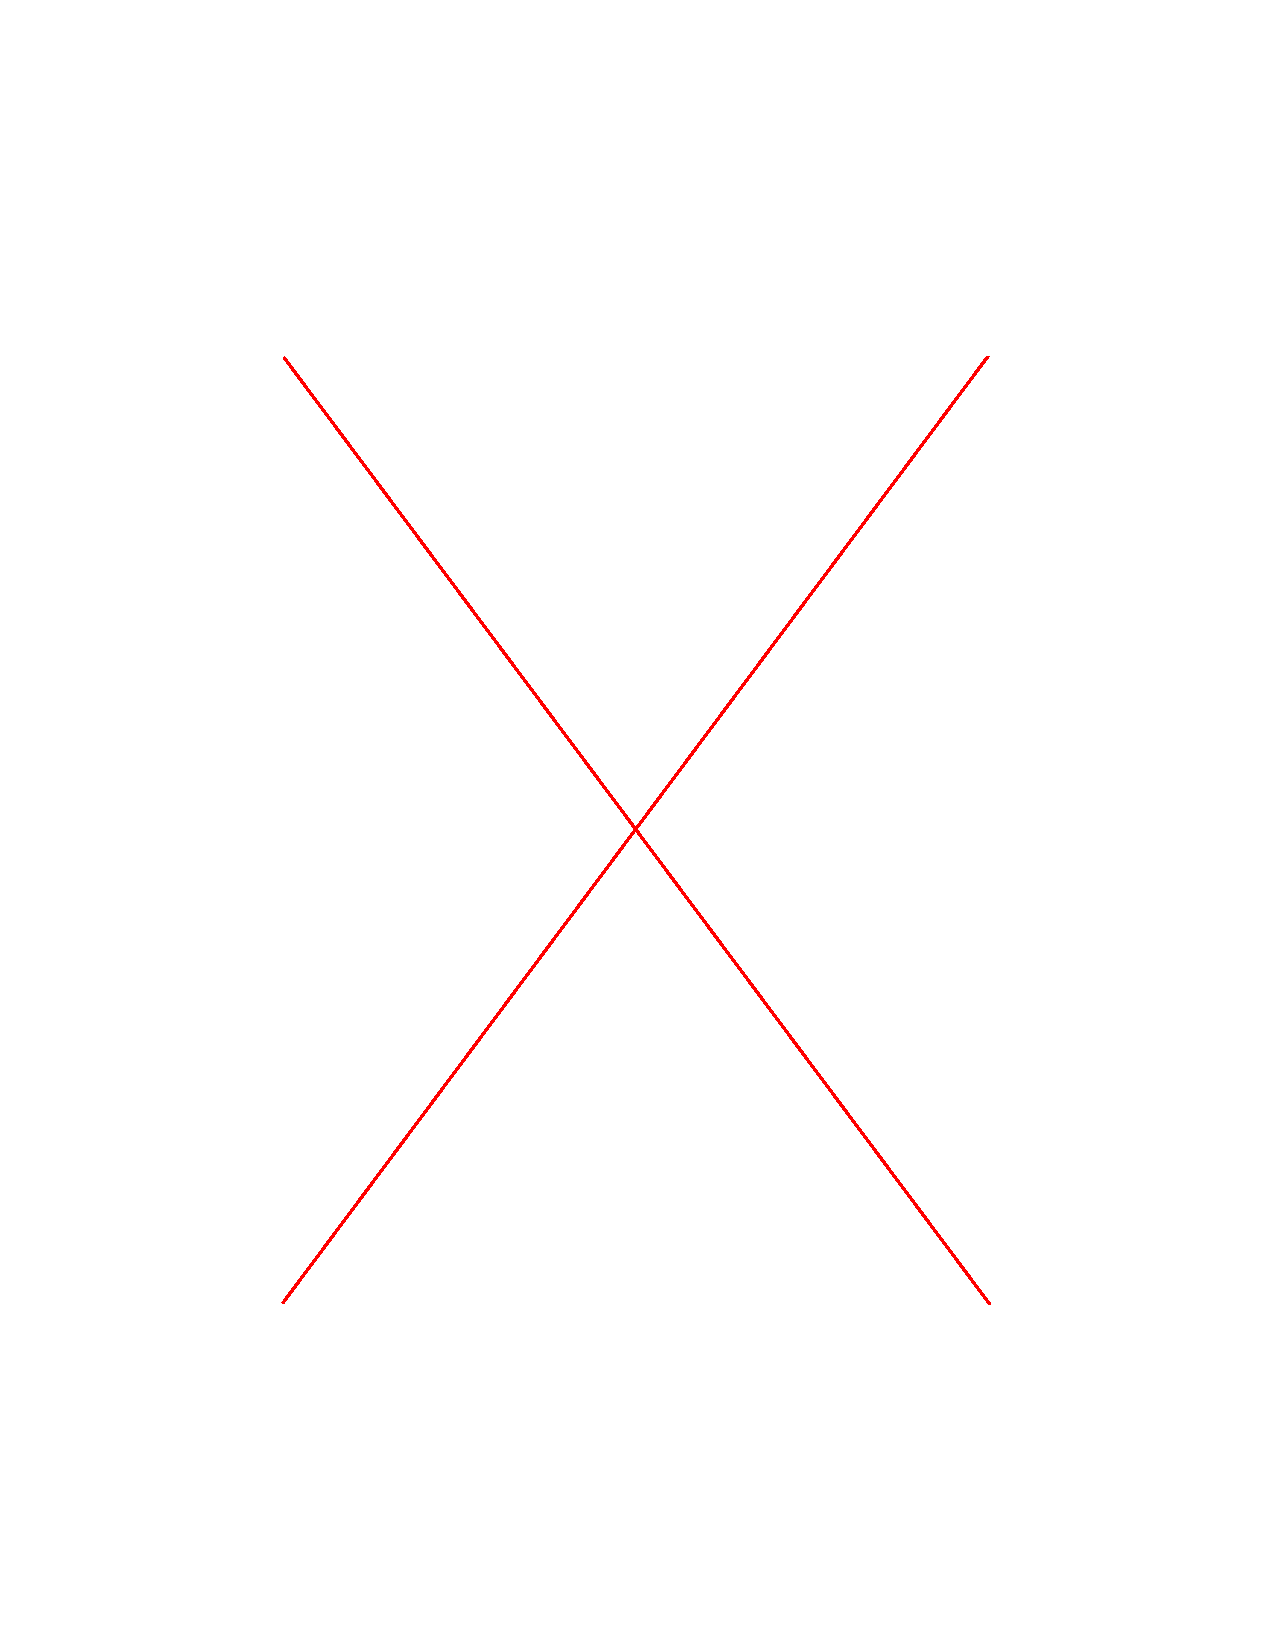
\includegraphics[width=0.4\textwidth]{small_fig} } \\
    \subfloat[]{ 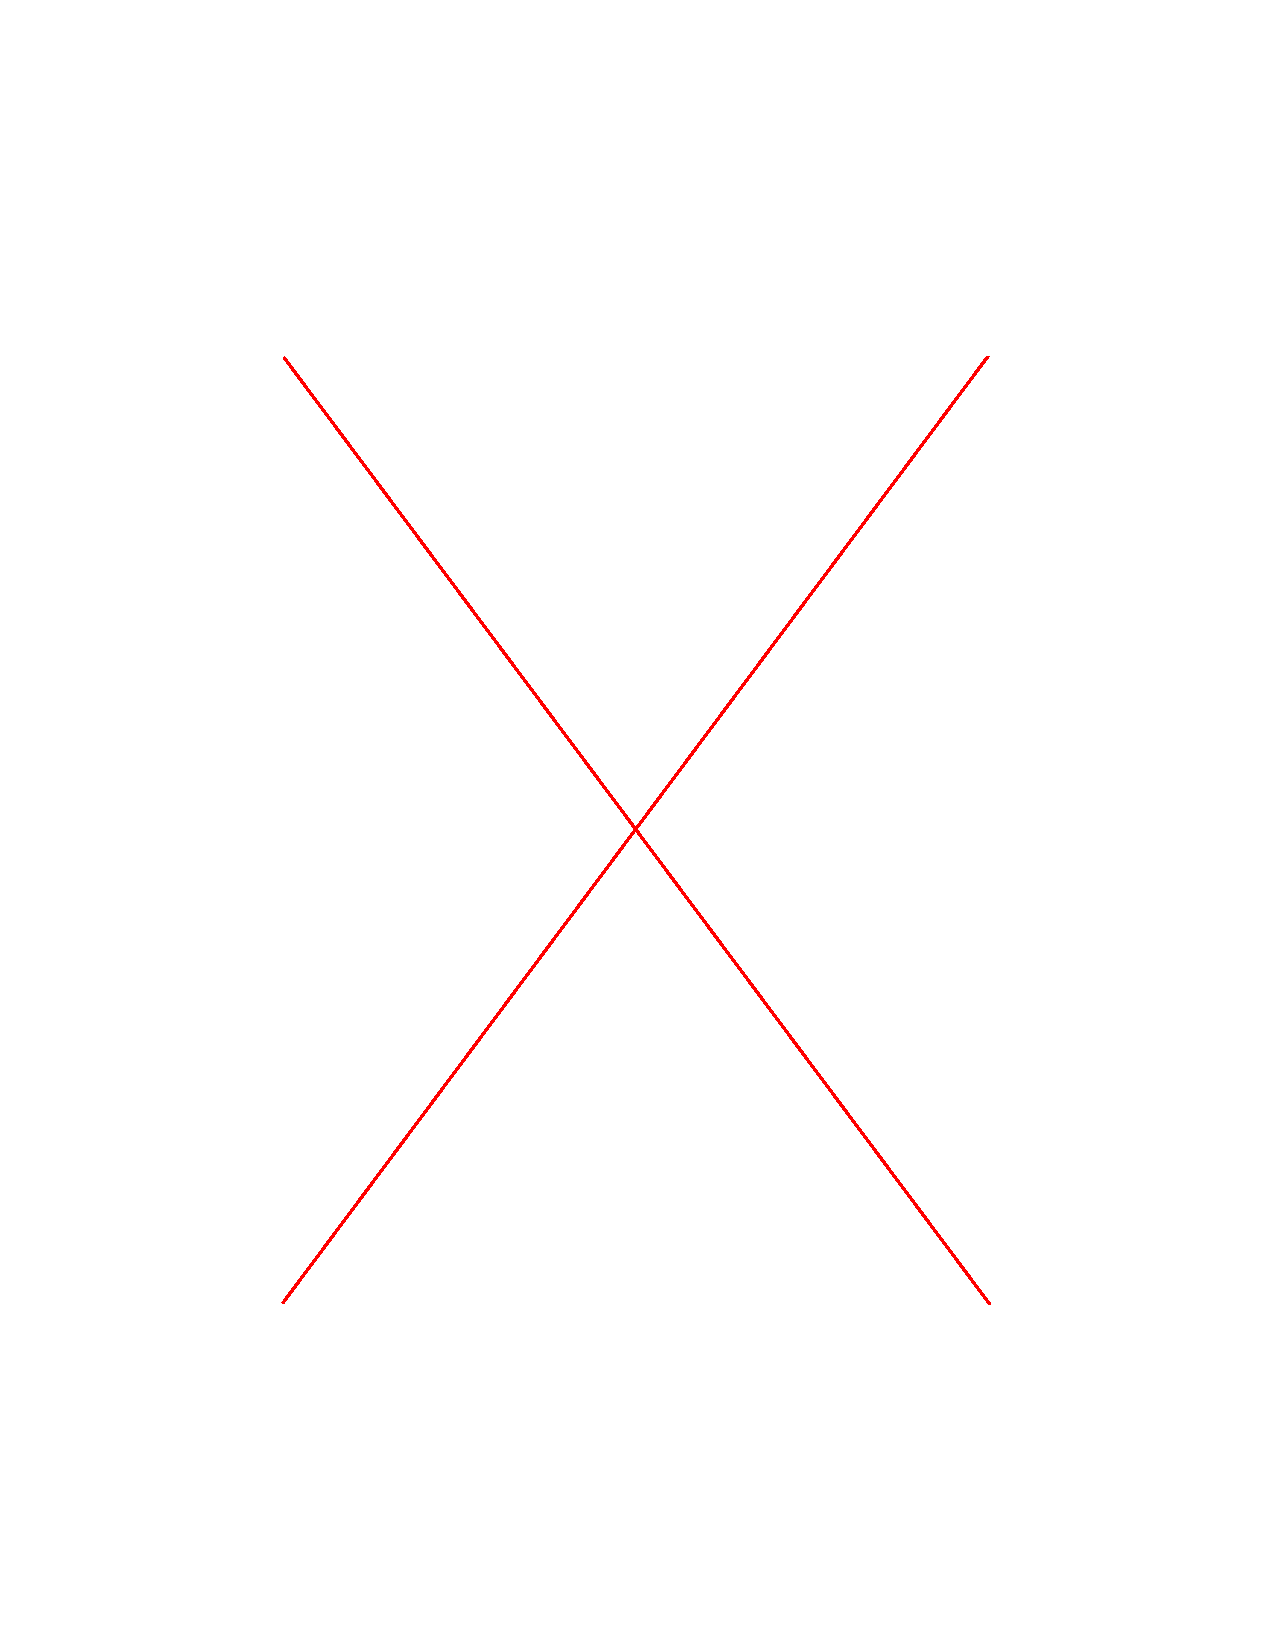
\includegraphics[width=0.4\textwidth]{small_fig} }
   \hfill
    \subfloat[]{ 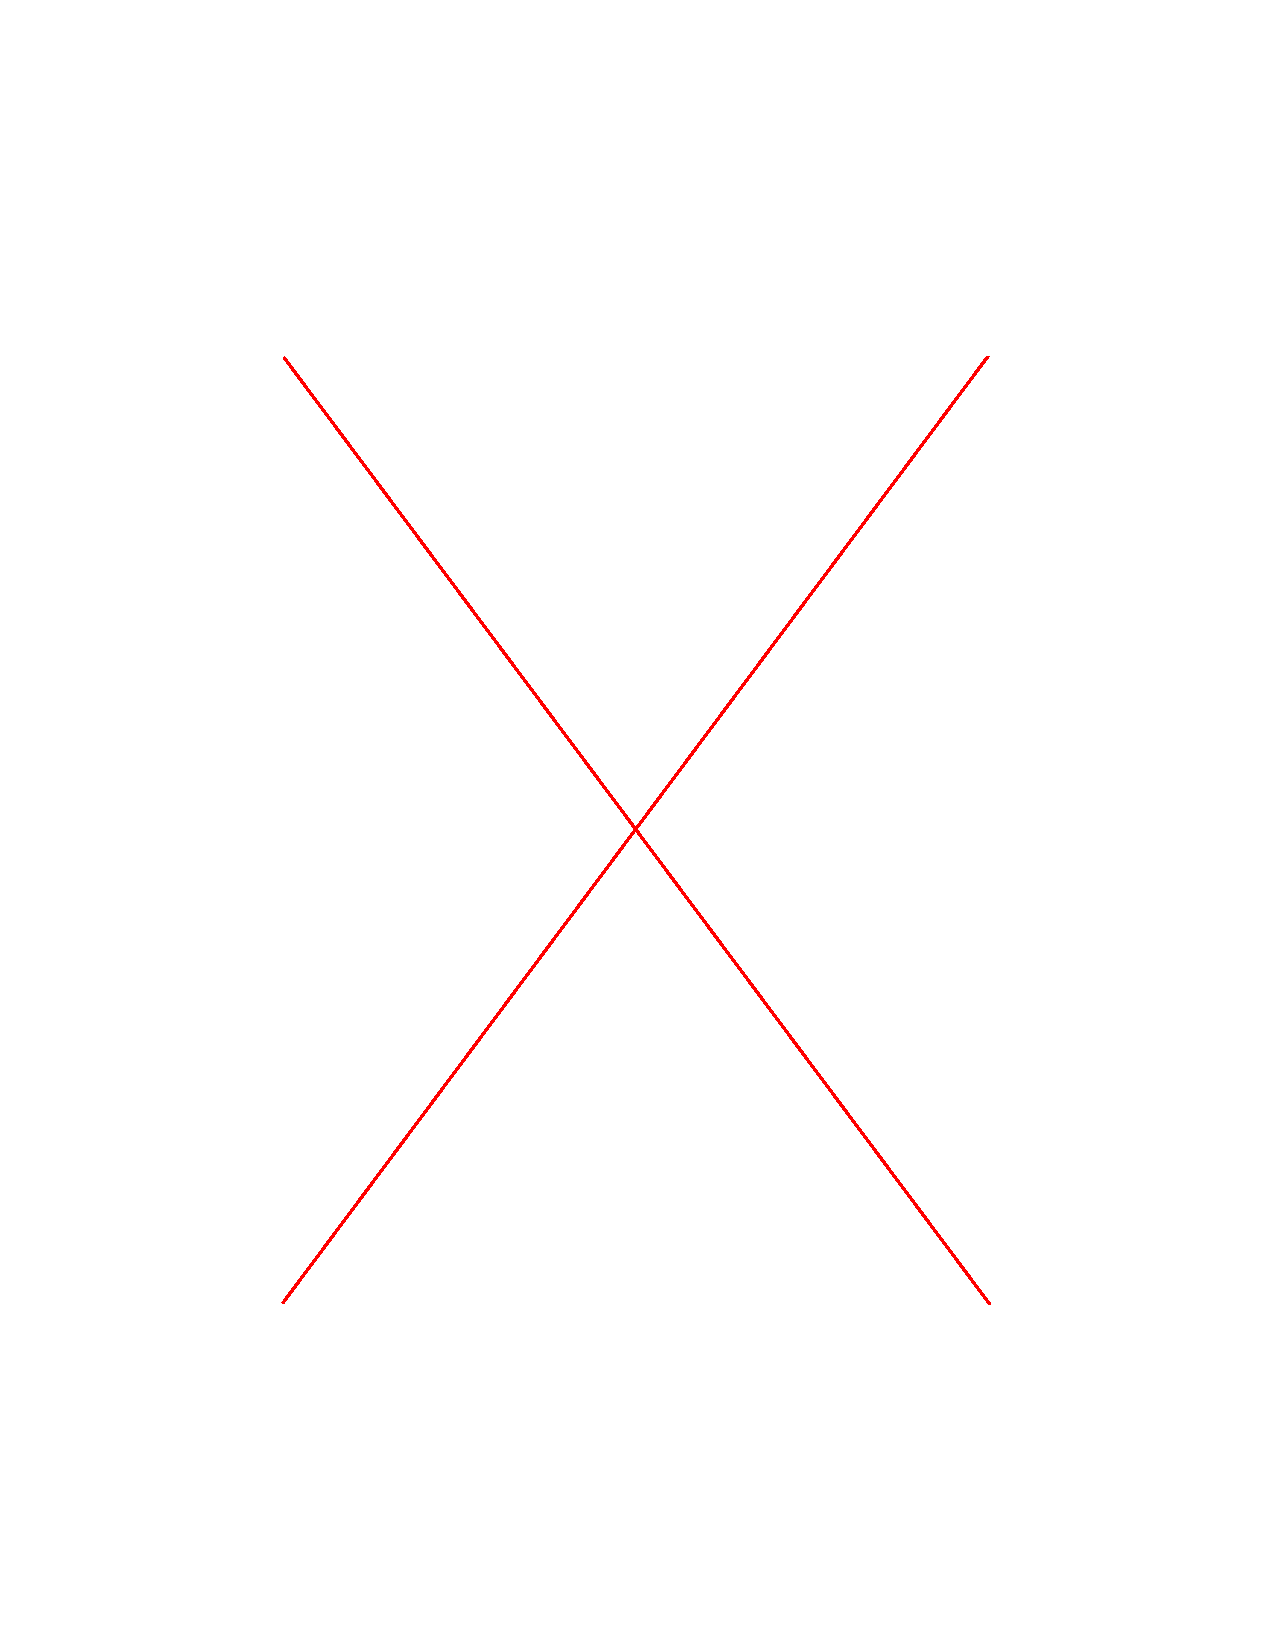
\includegraphics[width=0.4\textwidth]{small_fig} }\\
\caption{A full page of figures!}
\label{fig:full_page_fig}
\end{figure}

\chapter{Let's talk tables}
\label{chap:tables}

A simple table, with my personal tastes on borders and widths is shown below. 
\begin{table}[!htbp]
\begin{center}
\caption{Sequential modes in four-arm sinuous antennas.} 
\label{table:4sinuous_modes}
\def\arraystretch{1.5}
\begin{tabular}{|c | c | c | c | c |}
 \hline
Mode number & Port 1 & Port 2 & Port 3 & Port 4 \\
\hline
$M_{-2}$ & $0^\circ$ & $-180^\circ$ & $0^\circ$ & $-180^\circ$ \\ \hline
$M_{-1}$ & $0^\circ$ & $-90^\circ$ & $-180^\circ$ & $-270^\circ$ \\ \hline
$M_{+1}$ & $0^\circ$ & $90^\circ$ & $180^\circ$ & $270^\circ$ \\ \hline
$M_{+2}$ & $0^\circ$ & $180^\circ$ & $0^\circ$ & $180^\circ$ \\  \hline
\end{tabular}
\end{center}
\end{table}

\newpage

All the usual features of \LaTeX are possible, such as merging cells, wrapping / aligning text etc ...

\begin{table}[!h]
\begin{center}
\caption{Role of design parameters in sinuous antennas.}
\label{table:sinuous_design_roles}
\def\arraystretch{1.5}
\begin{tabular}{ | c | l | l | p{4cm} |}
 \hline
    Parameter & Denotes 		& Typical values 							& Role \\ \hline
    $N$ 	& Number of arms 	& $4$, $6$, $8$ 							& \parbox{4cm}{\vspace{1.5ex} Determines the number of modes obtainable.\vspace{1.5ex}} \\ \hline
    $R_1$ 	& Outer radius 	& $\frac{\lambda_L}{2\pi}$ to $\frac{\lambda_L}{3\pi/4}$ 	& \parbox{4cm}{\vspace{1.5ex} Sets the lower frequency limit.\vspace{1.5ex}}\\ \hline
    $\tau$ 	& Growth factor	& 0.6 to 0.9								& \parbox{4cm}{\vspace{1.5ex} Controls the ratio between adjacent cells and number of cells given a fixed size. \vspace{1.5ex}} \\ \hline    
    \multirow{2}{*}{$\alpha$} 	& \multirow{2}{*}{Angular span} 	&  \multirow{2}{*}{$22.5^\circ$ to $90^\circ$}					& \\  
    					&						&												& \\ \cline{1-3}
    \multirow{2}{*}{$\delta$} 	& \multirow{2}{*}{Angular spacing} 	&  \multirow{2}{*}{$11.25^\circ$ to $45^\circ$ }					& \multirow{-3}{4cm}{\strut These two parameters together control the angular span, interleaving and input impedance of the antenna.\vspace{1.5ex}} \\ 
   		&			&									& \\ \hline  
\end{tabular}
\end{center}
\end{table}

Finally, a large table, represented in landscape mode is shown in the next page.

\clearpage
\begin{landscape}
\begin{table}[!htbp]
\begin{center}
\caption{Review of performances of various broadband antennas.} 
\label{table:ant_summary}
\def\arraystretch{1.5}
\begin{tabular}{| l | p{4cm} | p{4cm} | p{4cm} | p{4cm} |}
\hline
\multicolumn{1}{|c|}{Aspect} & \multicolumn{1}{c|}{\pbox{4cm}{\vspace{1.5ex} Dipole-based designs (biconical, discone, ...)\vspace{1.5ex}} } & \multicolumn{1}{c|}{LPDA} & \multicolumn{1}{c|}{Spiral} & \multicolumn{1}{c|}{Sinuous} \\ 
\hline
Frequency bandwidth & Typically max at around two octaves. & Comparable to dipole-based designs, extendable by increasing elements. & Ratios of up to $40:1$ are possible. & Ratios comparable to spiral designs. \\ \hline
Multiple Polarization & Only possible if crossed elements are added. & Only possible if crossed elements are added. &  Possible with cavity-backing. & Possible with reconfigurable feed network. \\ \hline
Planar & Planar versions possible with maximum extents of order $\lambda/2$. & 3-D array of dipole ($\lambda/2$) sized elements with maximum extent determined by required bandwidth. & Planar versions possible with extent of order of $\lambda$ & Planar versions possible with extent of order of $\lambda$ \\ \hline
Radiation pattern & Cavity required for unidirectional radiation. & Cavity not required for unidirectional radiation. & Cavity required for unidirectional radiation. & Cavity required for unidirectional radiation.  \\ \hline
\end{tabular}
\end{center}
\end{table}
\end{landscape}

\chapter{Equations and code}
\label{chap:equationsandcode}

% --------------------------------------------------
% End of chapters
% --------------------------------------------------
% To add a symbol (no checking of repeated symbol)
\addsymbol{$\lambda$}{wavelength}
\addsymbol{$\epsilon_r$}{relative dielectric constant}
\addsymbol{$k$}{wave number, defined as $2\pi/\lambda$}

% To add an abbreviation, which will be named at least once in the full
\addabbrev{IEEE}{Institute of Electrical and Electronics Engineers}
\addabbrev{PASS}{Phased Array System Simulator}
\addabbrev{RF}{Radio Frequency}

% --------------------------------------------------
% Bibliography
% --------------------------------------------------
\bibliographystyle{IEEETran}
\bibliography{IEEEabrv,references_list}

\backmatter

\end{document}
